\documentclass{article}
\usepackage[utf8]{inputenc}
\usepackage[protrusion=true, expansion=true]{microtype}
\usepackage[hang, small, labelfont=bf, up, textfont=it, up]{caption}
\usepackage{listings}
\usepackage{ragged2e}
\usepackage{amsfonts}
\usepackage[font=small,labelfont=bf]{caption} % Required for specifying captions to tables and figures

\usepackage{csvsimple} 
\usepackage{color}


\usepackage{algpseudocode}
\usepackage{algorithm}

\usepackage{changepage}

\usepackage{graphicx}
\usepackage{amsmath}
\usepackage{fancyhdr}
\usepackage[a4paper, total={7in, 10in}]{geometry}
\usepackage[ddmmyyyy]{datetime}
\usepackage{lipsum}

\usepackage{tikz}
\usepackage{tikz-qtree}
\usepackage{amsmath,bm,times}
\usetikzlibrary{shapes,arrows,calc,arrows.meta}
\usetikzlibrary{decorations.pathreplacing,positioning, calc,shapes.multipart,chains,arrows}
\tikzset{listnode/.style={rectangle split, rectangle split parts=2,
    draw, rectangle split horizontal}}
\tikzset{hashtable/.style={rectangle split, rectangle split parts=5,
    draw, rectangle split}}
 
\usetikzlibrary{positioning}

\tikzset{
node of list/.style = { 
             draw, 
             fill=blue!20, 
             minimum height=6mm, 
             minimum width=6mm,
             node distance=6mm
   },
link/.style = {
     -stealth,
     shorten >=1pt
     },
array element/.style = {
    draw, fill=white,
    minimum width = 6mm,
    minimum height = 10mm
  }
}
\tikzset{main node/.style={circle,fill=blue!20,draw,minimum size=1cm,inner sep=0pt},
            }
    
\newcommand{\mx}[1]{\mathbf{\bm{#1}}} % Matrix comman2
\newcommand{\vc}[1]{\mathbf{\bm{#1}}} % Vector command

% We need layers to draw the block diagram
\pgfdeclarelayer{background}
\pgfdeclarelayer{foreground}
\pgfsetlayers{background,main,foreground}
% Define a few styles and constants
\tikzstyle{sensor}=[draw, fill=blue!20, text width=5em, 
text centered, minimum height=3.5em]
\tikzstyle{ann} = [above, text width=6em]
\tikzstyle{naveqs} = [sensor, text width=6em, fill=red!20, minimum width=7em,
minimum height=8em, rounded corners]




%Opening
\title{Trabalho Prático 2 - Coloração de Grafos}
\author{João Correia Costa (2019029027)}
\date{Novembro de 2023, Belo Horizonte}

\begin{document}

\maketitle

\section{Introdução}

Uma variedade de problemas na computação e na ciência podem ser modelados através de entidades e relações. Tal modelagem é comumente representada por meio de grafos coloridos que codificam as propriedades intrínsecas do sistema.

Nesse contexto, o presente trabalho busca validar a coloração de grafos, identificando se ela foi gerada por meio de um algoritmo guloso, ou seja, se um vértice \(v\) possui coloração \(i\), então ele possui pelo menos um vizinho com cada uma das cores menores que \(i\).

Tecnicamente, seja \(G = (V, E)\) um grafo \(k\)-colorível e \(c\) uma \(k\)-coloração própria de \(G\), a coloração \(c\) será gulosa se: \(\forall v \in V(G)\), se \(c(v) = i\) onde \(0 < i \leq k\) com \(0 < j < i\), existe um vértice \(u\) vizinho de \(v\) com \(c(u) = j\).

Para solucionar o problema, os grafos foram modelados através de um array, como lista de adjacência, combinada com listas simplesmente encadeadas. A escolha de um array de tamanho fixo foi possível, pois sabemos de antemão o tamanho \(N\) do grafo a ser validado. As listas encadeadas armazenam o índice dos vizinhos associados ao vértice de índice correspondente a sua posição em array. Essa implementação será descrita em mais detalhes na seção seguinte. A priori, para validar o grafo, percorremos a estrutura array+lista-encadeada observando se a coloração gulosa é satisfeita.

A segunda etapa do problema consiste em ordenar os vértices por cor, em primeiro, e por índice em segundo. Aplicamos os algoritmos de ordenação clássicos:  \texttt{bubble sort}, \texttt{selection sort}, \texttt{insertion sort}, \texttt{quick sort}, \texttt{merge sort}, \texttt{heap sort} e \texttt{count sort}, considerando o critério de ordenação citado. O objetivo consiste em analisar a performance desses algoritmos na ordenação dos vértices. Para isso, foram gerados grafos de tamanhos variados, medido o tempo de ordenação para cada algoritmo para construção de gráficos.


% Método
\section{Método}

\subsection{Estrutura de Dados}

A entrada de dados consiste em um inteiro $N$, que representa o tamanho do grafo. Subsequentemente, linha por linha, são fornecidos outros inteiros indicando o número de vizinhos para o vértice cujo índice corresponde ao número da linha. Por exemplo, a primeira linha descreve os vizinhos do vértice 0, a segunda linha descreve os vizinhos do vértice 1, e assim por diante. Após as $N$ linhas que descrevem os vizinhos, há uma linha adicional que representa a coloração de cada vértice.

Para armazenar essas informações de maneira eficiente, é apropriado utilizar um array de tamanho $N$ que contém ponteiros para listas encadeadas. Em outras palavras, na posição 0 em array, encontramos um ponteiro para uma instância da classe \texttt{Vertex} que descreve o vértice 0. Cada vértice é modelado por meio da classe \texttt{Vertex}, que é uma classe derivada da \texttt{LinkedList}. Além dos ponteiros comuns em listas encadeadas, que representam os índices dos vizinhos, a classe \texttt{Vertex} também armazena informações como a cor do vértice e o número de vizinhos. A representação gráfica dessa estrutura é exemplificada na figura abaixo.



% hashtable e graph


\def\LinkedList#1{%
  \foreach \element in \list {
     \node[node of list, right = of aux, name=ele] {\element};
     \draw[link] (aux) -- (ele);
     \coordinate (aux) at (ele.east);
  } 
}

\begin{figure}
\begin{center}
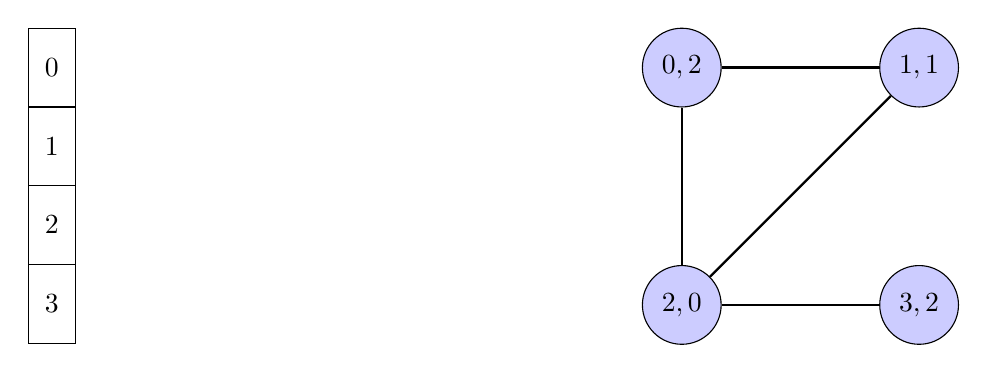
\begin{tikzpicture}

\foreach \index/\list in {0/{1, 2, null}, 1/{0, 2, null}, 2/{0, 1, 3, null}, 3/{2, null}} {
   \node[array element] (aux) at (0,-\index) {\index};
   \LinkedList{\list}
}

\begin{scope}[xshift=8cm]
    \node[main node] (1) {$0, 2$};
    \node[main node] (2) [right = 2cm of 1]  {$1, 1$};
    \node[main node] (3) [below = 2cm of 1] {$2, 0$};
    \node[main node] (4) [right = 2cm of 3] {$3, 2$};

    \path[draw,thick]
    (1) edge node {} (2)
    (1) edge node {} (3)
    (3) edge node {} (2)
    (3) edge node {} (4);
\end{scope}
\end{tikzpicture}
\end{center}
\caption{Array de Lista Encadeadas e Grafo(índice, cor)}
\end{figure}


% linked list double versus arrays


Alternativamente, poderia ter sido empregada uma lista encadeada dupla; no entanto, a escolha da estrutura de dados composta por uma array e uma lista encadeada oferece um desempenho superior neste contexto. Em primeiro lugar, a array representa um bloco contíguo de memória, resultando em um acesso mais eficiente a um elemento em qualquer índice. Embora se possa argumentar que a array possui uma estrutura mais rígida em comparação com a lista encadeada, essa rigidez não se configura como uma desvantagem significativa no contexto específico dos grafos fornecidos, pois esses  têm tamanho fixo.

Em segundo lugar, a combinação de uma array e uma lista encadeada proporciona flexibilidade em termos de tamanho, pois lista encadeada permite a alocação dinâmica de memória, adaptando-se de maneira eficaz ao número variável de vizinhos para cada vértice.

Assim, a escolha dessa estrutura de dados composta demonstra ser uma abordagem eficaz, otimizando o acesso e alocando dinamicamente recursos conforme necessário para representar o grafo.


\subsection{Validação}

A validação da coloração do grafo consiste em verificar se cada vértice \(v\) de cor \(i\) possui pelo menos um vizinho com cada uma das cores menores que \(i\). Cada vértice, representado pela classe \texttt{Vertex<int>}, é dotado de um método denominado \texttt{bool validate}. Essencialmente, esse método percorre a lista encadeada contendo os índices dos vizinhos de \(v\), busca a cor de cada vizinho na array de vértices \texttt{Vertex<int>** graph} e verifica se o conjunto de cores observado preenche todo o intervalo \([1, i)\).

A função auxiliar \texttt{bool validate\_graph}, presente no arquivo \texttt{utils.hpp}, realiza uma iteração sobre todos os vértices na array, invocando o método \texttt{validate} para cada vértice individual. O resultado final é conjunção de todos os valores retornados pelos vértices, indicando uma coloração válida caso a conjução seja verdadeira (retorna true).

\subsection{Ordenação}
Após a validação do grafo, procede-se à ordenação dos vértices primeiro por cor e, em seguida, por índice. A implementação dessas operações é clássica, uma vez que envolve a ordenação de valores inteiros que representam cores e índices. Para fins práticos, a troca de posição dos vértices é realizada através da manipulação dos ponteiros para os vértices. Em outras palavras, se o vértice 5 deve ser colocado antes do vértice 0, os endereços de memória desses vértices são trocados entre si.

A função \texttt{void swap\_vertex} é responsável por efetuar essa troca de endereços. Nesse contexto, a aplicação dos métodos de ordenação assemelha-se à ordenação de um vetor de inteiros. No entanto, em vez de acessar valores diretamente, utilizam-se getters para obter as cores e índices dos vértices, e a troca de posições é realizada manipulando os endereços de memória dos vértices.

Os métodos de ordenação aplicados são: \texttt{bubble sort}, \texttt{selection sort}, \texttt{insertion sort}, \texttt{quick sort}, \texttt{merge sort}, \texttt{heap sort} e \texttt{count sort}.
A descrição breve desses algoritmos consta na seção de análise de complexidade.

\section{Análise de Complexidade}
Essa seção se dedica a analisar a complexidade assintótica, em termos de espaço e de tempo, das principais funções envolvidas em validar a coloroção e ordenar o grafo.


\subsection{\texttt{bool validate\_graph}}
   \begin{itemize}
     \item O método itera sobre todos os n vértices do grafo (complexidade \(O(n)\)).
     \item Chama o método \texttt{validate} para cada vértice, o qual itera sobre os vizinhos (complexidade média \(O(\text{{grau do vértice}})\)).
     \item Portanto, a complexidade total é \(O(n \cdot \text{{grau médio}})\).
   \end{itemize}

\subsection{\texttt{bool Vertex::validate}}
   \begin{itemize}
     \item O método itera sobre as cores até \(\text{{target\_color}} = \_color - 1\).
     \item Para cada cor, itera sobre todos os vizinhos (complexidade média \(O(\text{{grau do vértice}})\)).
     \item Assim, a complexidade total é \(O(\_color \cdot \text{{grau médio}})\).
   \end{itemize}
   
 Se considerarmos grafos de densidade constante, isto é, o grau médio é fixo, a complexidade final do algoritmo é dominada por \texttt{validate\_graph}, resultando em uma complexidade média de \(O(n)\). Observa-se que como o grau do vértice é fixo, o número de cores é limitada, logo \texttt{Vertex::validate} performa um número pequeno e fixo de iterações, complexidade \(O(1)\).

% bubble sort
\subsection{\texttt{void bubble\_sort(Vertex<int>**\& graph, int n\_vertex)}}
\begin{itemize}
    \item O método itera sobre todos os \(n_{\text{vertex}}\) vértices do grafo (complexidade \(O(n_{\text{vertex}})\)).
    \item Para cada vértice, o loop interno itera sobre \(n_{\text{vertex}}-i-1\) outros vértices.
    \item A complexidade total é \(O(n_{\text{vertex}}^2)\).
\end{itemize}

O Bubble Sort tem custo de memória \(O(1)\), pois opera in-place.


% insertion sort
\subsection{\texttt{void insertion\_sort(Vertex<int>**\& graph, int n\_vertex)}}
\begin{itemize}
    \item O método itera sobre todos os \(n_{\text{vertex}}\) vértices do grafo (complexidade \(O(n_{\text{vertex}})\)).
    \item Para cada vértice, o loop interno executa um número variável de iterações, dependendo da posição correta do vértice na sequência ordenada até o momento.
    \item No pior caso, o número total de iterações do loop interno é \(O(i)\), onde \(i\) é o índice do vértice no array.
    \item A complexidade total do algoritmo é, portanto, \(O(n_{\text{vertex}}^2)\) no pior caso.
\end{itemize}

O Insertion Sort tem custo de memória \(O(1)\), pois opera in-place.

% Selection Sort

\subsection{\texttt{void selection\_sort(Vertex<int>**\& graph, int n\_vertex)}}
\begin{itemize}
    \item O método itera sobre todos os \(n_{\text{vertex}} - 1\) elementos do grafo (complexidade \(O(n_{\text{vertex}})\)).
    \item Para cada elemento na iteração externa, o loop interno encontra o índice do menor elemento na parte não ordenada do array (complexidade média \(O(n_{\text{vertex}})\)).
    \item A função \texttt{swap\_vertex} é chamada uma vez por iteração externa.
    \item A complexidade total do algoritmo é \(O(n_{\text{vertex}}^2)\).
\end{itemize}

O Selection Sort tem custo de memória \(O(1)\), pois opera in-place.

% Quick Sort

\subsection{\texttt{void quick\_sort(Vertex<int>**\& graph, int n\_vertex)}}
\begin{itemize}
    \item A função \texttt{quick\_sort} é uma implementação recursiva do algoritmo Quick Sort.
    \item A função principal \texttt{quick\_sort(graph, p, r)} chama a função \texttt{partition} para encontrar a posição do pivô.
    \item Em seguida, chama recursivamente \texttt{quick\_sort} para as partições à esquerda e à direita do pivô.
    \item A complexidade de tempo média do Quick Sort é \(O(n \log n)\), onde \(n\) é o número de elementos a serem ordenados.
    \item No pior caso, a complexidade é \(O(n^2)\), mas isso é raro na prática.
    \item A complexidade de espaço é \(O(n)\) devido às chamadas recursivas, tornando-o eficiente em termos de memória.
\end{itemize}


% Merge Sort

\subsection{\texttt{void merge(Vertex<int>** graph, int left, int mid, int right)}}
\begin{itemize}
    \item A função \texttt{merge} realiza a fusão de duas sub-arrays ordenadas em um único array ordenado.
    \item Calcula os tamanhos das sub-arrays (\(n1\) e \(n2\)).
    \item Cria sub-arrays temporárias \texttt{left\_arr} e \texttt{right\_arr}.
    \item Preenche as sub-arrays temporárias com os elementos correspondentes da array original.
    \item Combina as sub-arrays de volta na array original em ordem ordenada.
    \item A complexidade temporal é \(O(n \log n)\), onde \(n\) é o número total de elementos a serem ordenados.
    \item A complexidade espacial é \(O(n)\) devido às sub-arrays temporárias.
\end{itemize}


% Heap Sort

\subsection{\texttt{void heap\_sort(Vertex<int>**\& graph, int n\_vertex)}}
\begin{itemize}
    \item A função \texttt{heap\_sort} utiliza uma estrutura de heap para realizar a ordenação.
    \item Cria uma instância da classe \texttt{Heap} com capacidade inicial de \texttt{n\_vertex}.
    \item Insere os vértices no heap com base em uma tupla contendo a cor e o ID do vértice.
    \item Cria uma array temporária \texttt{sortedGraph} para armazenar os vértices ordenados.
    \item Reordena a array \texttt{sortedGraph} com base na ordem de remoção do heap.
    \item Copia os vértices ordenados de volta para a array original \texttt{graph}.
    \item A complexidade temporal do Heap Sort é \(O(n \log n)\), onde \(n\) é o número de elementos a serem ordenados.
    \item A complexidade espacial é \(O(n)\) devido à array temporária \texttt{sortedGraph}.
\end{itemize}


% Counting Sort

\subsection{\texttt{void count\_sort(Vertex<int>**\& graph, int n\_vertex)}}
\begin{itemize}
    \item A função \texttt{count\_sort} implementa o algoritmo de ordenação Counting Sort.
    \item Inicializa um array de contagem \texttt{count\_arr} de tamanho \(n\_vertex\) e o preenche com zeros.
    \item Conta a ocorrência de cada cor no grafo, incrementando os contadores em \texttt{count\_arr}.
    \item Realiza a contagem cumulativa em \texttt{count\_arr}.
    \item Cria um array temporário \texttt{output} para armazenar os elementos ordenados.
    \item Atribui os elementos de \texttt{graph} ao array \texttt{output} de acordo com a contagem cumulativa.
    \item Atualiza o array original \texttt{graph} com os elementos ordenados em \texttt{output}.
    \item Libera a memória alocada para o array temporário \texttt{output}.
    \item A complexidade temporal é \(O(n)\), onde \(n\) é o número total de vértices no grafo.
    \item A complexidade espacial é \(O(n)\) devido ao array de contagem \texttt{count\_arr} e ao array temporário \texttt{output}.
\end{itemize}




% Estratégias de Robustez

\section{Estratégias de Robustez}
Com o objetivo de tornar o programa mais robusto e evitar problemas com entradas inválidas, foram criadas classes de exceção \texttt{ExceptionEmptyList}. Essa exceção é disparada, com uma mensagem de erro descritiva, caso a função de remoção de um elemento da lista seja invocada para uma estrutura vazia. 

Para manter a integridade do programa e evitar vazamentos de memória, todos os Tipos Abstratos de Dados (TADs) implementam destrutores apropriados. Nos destrutores da lista encadeada, garantimos que o estado da instância retorne ao \texttt{default} e \texttt{asserts} checam se o tamanho da estrutura é zero.

Além disso, foram realizados testes com o Valgrind, e nenhum erro relacionado à alocação de memória foi observado.

Entretanto, é importante destacar que o programa ainda possui limitações, uma vez que não cobre um amplo espectro de possíveis entradas de dados, presumindo que o usuário fornecerá entradas corretas. 


\section{Análise Experimental}

\subsection{Algoritmos de Ordenação}
O presente experimento foi conduzido com o propósito de avaliar o custo computacional de diferentes algoritmos de ordenação. Foram gerados 29 grafos, variando o número de vértices de 1000 a 30000. A quantidade de arestas em cada grafo foi estabelecida como 50\% superior ao número de vértices. O tempo de execução de cada algoritmo de ordenação foi medido em relação a esses grafos, utilizando a biblioteca \texttt{chrono}. Os resultados temporais obtidos foram então representados graficamente, conforme ilustrado na Figura no Apêndice B.



Ao analisar o gráfico, destacam-se três grupos de desempenho. O grupo de pior desempenho inclui os algoritmos \texttt{bubble\_sort} e \texttt{selection\_sort}; em segundo lugar, temos o \texttt{insertion\_sort}; e o terceiro grupo engloba os demais algoritmos, que apresentam um custo temporal abaixo de décimos de segundo para todos os grafos.

Presume-se que o desempenho superior do \texttt{insertion\_sort} em relação ao primeiro grupo deve-se à sua adaptabilidade a dados parcialmente ordenados, ou seja, os grafos fornecidos já possuem uma ordenação razoável. Os algoritmos do primeiro grupo não se beneficiam da ordenação parcial.

Como esperado, os algoritmos \texttt{merge\_sort}, \texttt{heap\_sort}, \texttt{quick\_sort} apresentaram desempenho muito superior aos outros grupos, especialmente para grafos grandes. Isso pode ser explicado, em primeiro lugar, pela função de complexidade desses três algoritmos, que no pior caso é \(O(n \log n)\) para o \texttt{merge\_sort} e \texttt{heap\_sort}, e \(O(n^2)\) para o \texttt{quick\_sort}, embora geralmente o \texttt{quick\_sort} apresente \(O(n \log n)\), conforme observado no gráfico.

Além disso, o uso de estruturas de dados auxiliares, como Heaps e arrays extras, também contribuem para a eficiência desses três algoritmos.

No grupo de melhor desempenho, é destacado um terceiro algoritmo de ordenação: o Count Sort. O Count Sort é eficiente para conjuntos de dados com um intervalo pequeno de valores, como é o caso dos grafos do experimento, que têm uma faixa limitada de cores. Sua complexidade temporal é linear \(O(n)\), onde \(n\) é o número de vértices, o que o torna uma escolha eficiente para o problema proposto.


\subsection{Validação}

Ao analisarmos o tempo de execução da função de validação da coloração dos grafos, observamos uma curva linear, o que está em conformidade com a análise de complexidade \(O(n)\). A Figura correspondente pode ser encontrada no Apêndice B.
Essa análise é fundamentada na compreensão da complexidade dos métodos envolvidos na validação da coloração: \texttt{bool validate\_grapgh} e \texttt{bool validate}.




\section{Conclusões}

No projeto, abordamos o problema clássico de coloração em grafos, com ênfase na complexidade algorítmica e nas estruturas de dados implementadas em C++. Inicialmente, desenvolvemos um algoritmo para identificar se a coloração do grafo é gulosa, isto é, se um vértice \(v\) possui coloração \(i\), então ele possui pelo menos um vizinho com cada uma das cores menores que \(i\). Em seguida, aplicamos algoritmos clássicos de ordenação, seguindo o critério de cor e índice, conforme descrito na função \texttt{bool criterium}.

Ao longo do projeto, aprofundamos nosso entendimento das estruturas de dados eficientes para modelagem de grafos, como a combinação de array e lista encadeada. Também exploramos os algoritmos de ordenação clássicos, destacando as nuances entre suas complexidades assintóticas em termos de tempo e memória.

Este trabalho não apenas ampliou nossa habilidade de implementar soluções algorítmicas em C++, mas também proporcionou insights sobre a escolha e aplicação de estruturas de dados e algoritmos em cenários específicos, contribuindo para uma compreensão mais abrangente da ciência da computação.





\section{Bibliografia}
1. Chaimowicz, L. and Prates, R. (2020). Slides virtuais da disciplina de estruturas de dados. Disponibilizado via moodle. Departamento de Ciência da Computação. Universidade
Federal de Minas Gerais. Belo Horizonte. 
\justify
2. Introduction to Algorithms, Thomas H. Cormem, Charles E. Leiserson, Ronald L. Rivest.




\appendix
\newpage
\section{Instruções para Compilação e Execução}
\label{ap:compilacao_execucao}

\textbf{Observação:} Certifique-se de que você tenha o compilador GCC (g++) instalado em seu sistema para a compilação.

\subsection{Compilação do Projeto}

Para compilar o projeto, siga as instruções abaixo:

\begin{enumerate}
    \item Abra um terminal e navegue até o diretório raiz do projeto.
    \item Certifique-se de que o projeto contenha a seguinte estrutura de diretórios:
    
    \begin{verbatim}
    - src/
    - obj/
    - bin/
    - include/
    \end{verbatim}

    \item Utilize o seguinte comando para compilar o projeto:

    \begin{verbatim}
    make ou make all
    \end{verbatim}

    Isso irá compilar o projeto e gerar o executável \texttt{bin/tp2.out}.

\end{enumerate}

\subsection{Execução do Projeto}

Para executar o projeto compilado, utilize o seguinte comando:

\begin{verbatim}
./bin/tp2.out
\end{verbatim}

Este comando executará o programa principal.


\subsection{Limpeza dos Arquivos Compilados}

Para limpar os arquivos compilados e executáveis, utilize o seguinte comando:

\begin{verbatim}
make clean
\end{verbatim}

Isso removerá os arquivos objetos e executáveis.

\newpage
\section{Figuras}

\begin{figure}[H]
    \begin{minipage}{\textwidth}
        \centering
        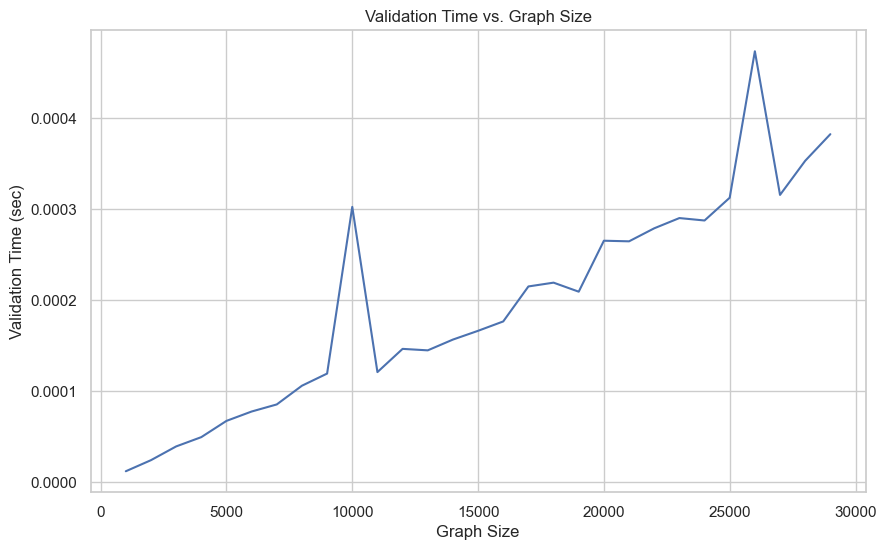
\includegraphics[width=0.8\linewidth]{~/Documents/UFMG-CODE/graphColoration/experiments/validation_time_vs_graph_size.png}
        \caption{Desempenho da função de validação dos grafos do experimento.}
        \label{fig:validacao}
    \end{minipage}
\end{figure}

\vspace{1cm}

\begin{figure}[H]
    \begin{minipage}{\textwidth}
        \centering
        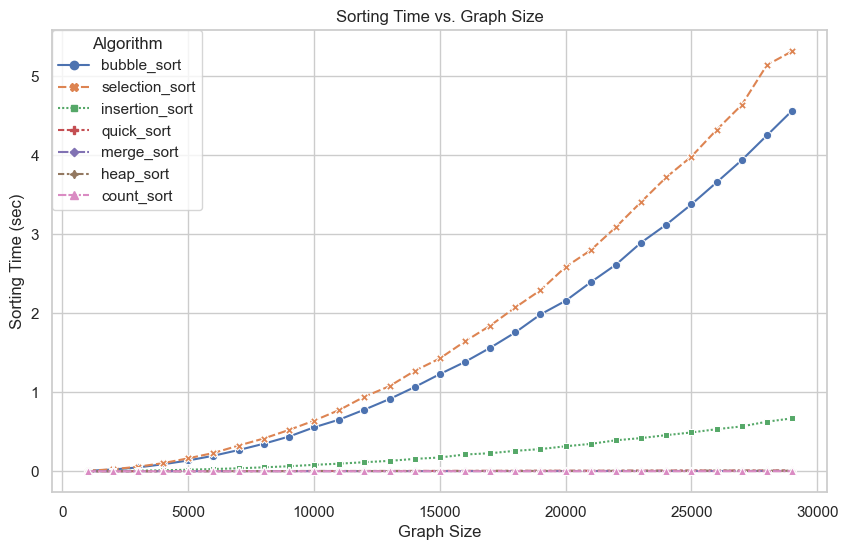
\includegraphics[width=0.8\linewidth]{~/Documents/UFMG-CODE/graphColoration/experiments/sorting_time_vs_graph_size.png}
        \caption{Desempenho dos algoritmos de ordenação para os grafos do experimento.}
        \label{fig:ordenacao}
    \end{minipage}
\end{figure}

\label{ap:figuras}


\end{document}
